\documentclass[11pt,a4paper]{article}
\usepackage[a4paper,top=22mm,bottom=22mm,left=23mm,right=23mm]{geometry}
\usepackage{fontspec}
\setmainfont{Times New Roman}
\usepackage{microtype,amsmath,graphicx,booktabs,tabularx,array,longtable}
\usepackage{caption,fancyhdr,titlesec,xcolor,url}
\usepackage[hidelinks]{hyperref}
\definecolor{navy}{HTML}{17394B}
\definecolor{teal}{HTML}{176D79}
\definecolor{soft}{HTML}{EAF1F2}
\titleformat{\section}{\large\bfseries\color{navy}}{\thesection}{0.6em}{}
\titleformat{\subsection}{\normalsize\bfseries\color{teal}}{\thesubsection}{0.6em}{}
\titlespacing*{\section}{0pt}{13pt}{5pt}
\titlespacing*{\subsection}{0pt}{9pt}{3pt}
\captionsetup{font=small,labelfont=bf}
\setlength{\parindent}{1em}
\setlength{\parskip}{3pt}
\renewcommand{\arraystretch}{1.15}
\pagestyle{fancy}
\fancyhf{}
\fancyhead[L]{\footnotesize SeaNergy | India Cost and Market Analysis}
\fancyhead[R]{\footnotesize SIH 26058}
\fancyfoot[C]{\footnotesize \thepage}
\renewcommand{\headrulewidth}{0.3pt}
\newcolumntype{Y}{>{\raggedright\arraybackslash}X}
\begin{document}
\begin{center}
{\color{teal}\rule{\textwidth}{1.1pt}}\par\vspace{3mm}
{\fontsize{19}{22}\selectfont\bfseries Techno-Economic Assessment and India Market Sizing for the SeaNergy Adaptive Sonar Payload\par}
\vspace{2mm}
{\large Cost structure, TAM--SAM--SOM, pricing, and sensitivity | SIH 26058\par}
\vspace{3mm}{\color{teal}\rule{\textwidth}{0.4pt}}
\end{center}

\noindent\textbf{Abstract.} This paper converts the SeaNergy project bill of materials and market workbook into a transparent India-focused commercial model. A narrow global side-scan sonar category provides a 2025 total addressable market (TAM) proxy of INR 452.30 crore at a stated INR 95.7245/USD planning rate. A five-year Indian serviceable available market (SAM) is built bottom-up from 174 estimated opportunities across five customer groups, totaling INR 31.92 crore. A qualification-led serviceable obtainable market (SOM) scenario assumes 35 integrated-payload engagements worth INR 6.61 crore over five years. These are planning estimates, not sales orders. The entry evaluation-unit target is INR 1,95,000 ex-GST against estimated cost of goods sold (COGS) of INR 1,17,648, producing INR 77,352 unit gross profit and 39.7\% gross margin. Integrated packages in the SOM are a different offer and do not inherit this unit margin. Component, scale, pricing, exchange-rate, and programme-spend sensitivities are quantified. Government programme budgets and supplier list prices provide context but are not booked as SeaNergy revenue. The method, assumptions, and sources are disclosed so every number can be updated as quotations and qualification evidence arrive.\par
\noindent\textbf{Keywords:} underwater technology; AUV; India; sonar; bill of materials; TAM; SAM; SOM; unit economics; procurement.\par

\section{Decision Summary}
\begin{table}[htbp]\centering
\begin{tabularx}{\textwidth}{@{}Yrr@{}}
\toprule
Indicator & Value & Basis\\ \midrule
Narrow global TAM proxy, 2025 & INR 452.30 crore & Published category estimate, fixed FX\\
India five-year SAM & INR 31.92 crore & 174 estimated serviceable units\\
Five-year staged SOM & INR 6.61 crore & 35 projected integrated engagements\\
Evaluation unit target price & INR 1,95,000 & Ex-GST planning price\\
Evaluation unit estimated COGS & INR 1,17,648 & Seven cost elements\\
Evaluation unit gross margin & 39.7\% & Before programme overhead\\
Field-stage scaling reserve & INR 14.35 lakh & Engineering allowance\\ \bottomrule
\end{tabularx}
\caption{The model's main figures. Market opportunities, unit economics and capital allowances have different definitions and are not added together.}
\label{tab:dashboard}
\end{table}

The commercial thesis is a programmable Indian acoustic transmitter/payload path for research, inspection and AUV/ROV integration. The product has a potential wedge in transparent waveform choices, local integration and low-duty operation. It should not be presented as a direct substitute for every scanning, multibeam or mature side-scan imager. Qualification, calibrated pressure and acoustic evidence, procurement cycles and repeatable production limit early capture.

\section{Method and Product Boundary}
\subsection{Two offers, two cost questions}
The project workbook contains an evaluation-unit price of INR 1.95 lakh and a separate five-year sales scenario with average selling prices (ASPs) from INR 15 to 20 lakh. These are not the same SKU. The lower-priced offer is a controller and acoustic evaluation kit with local support; the higher-priced opportunity is an integrated payload or paid programme containing vehicle interfacing, ruggedized packaging, acoustic-chain development, calibration, installation, documentation and support. The workbook gives a component-level COGS for the former. It does not yet give signed quotations or a full COGS for the latter. This distinction prevents an attractive kit margin from being incorrectly applied to integrated systems.

\begin{table}[htbp]\centering
\begin{tabularx}{\textwidth}{@{}p{0.20\textwidth}YY@{}}
\toprule
Commercial item & Included commercial scope & Model treatment\\ \midrule
Bench demonstrator & Electronics and assembly for one prototype & INR 27,648 quantity-one bill; INR 36,000 demonstration envelope\\
Evaluation unit & Controller, integrated acoustic parts, enclosure, battery, calibration, warranty reserve and field kit & INR 1,95,000 ex-GST price; INR 1,17,648 COGS\\
Integrated programme & Payload adaptation, vehicle/mission integration, calibration and support & INR 15--20 lakh staged ASP; revenue scenario only\\
Field-stage development & Pressure housing, higher-power drive, calibrated instrumentation and integration & INR 14.35 lakh programme reserve\\ \bottomrule
\end{tabularx}
\caption{Product and accounting boundaries. The unit price, SOM ASP and development reserve are intentionally separate.}
\label{tab:tiers}
\end{table}

\subsection{Equations and source hierarchy}
For a category estimate $M_{\rm USD}$ in USD million and FX rate $x$ INR/USD,
\begin{equation}
TAM_{\rm INR,cr}=M_{\rm USD}\,x/10.
\label{eq:tam}
\end{equation}
The divisor converts INR million to INR crore. The Indian segment model is
\begin{equation}
SAM_{\rm cr}=\frac{\sum_i U_i A_i}{100},
\quad
SOM_{\rm cr}=\frac{\sum_y u_y a_y}{100},
\label{eq:sam}
\end{equation}
where $U_i$ and $u_y$ are estimated unit counts, and $A_i$ and $a_y$ are ASPs in INR lakh. A crore equals 100 lakh. The segmentation and capture counts are team planning assumptions; published government outlays validate application context, not SeaNergy purchases.

Source priority is: project BOM and cost workbook for internal design costs \cite{bom,workbook}; official Government of India releases for public programmes \cite{dom,aditi,sagarmala}; product makers for public comparison prices \cite{ping,echo}; and named category reports for global market estimates \cite{diresearch,gir}. All currency figures in the model use INR. Global prices and market estimates are translated with a stated rate rather than an unstated current conversion.

\section{Global TAM Proxy}
DIResearch describes a 2025 global side-scan sonar market of USD 47.25 million and 2032 estimate of USD 55.21 million \cite{diresearch}. A second, adjacent category, side-scan echo sounders, reports USD 49.01 million for 2025 \cite{gir}. At the workbook's INR 95.7245/USD rate dated 11 September 2026, these imply INR 452.30 crore and INR 469.15 crore respectively \cite{fx,workbook}. The selected TAM is the first figure, not an average. Its narrow category is more defensible than adding the entire ocean-technology or defence budget, yet it remains a proxy: SeaNergy initially sells a transmitter/controller and integration service, whereas many reported side-scan revenues include full receive and imaging systems.

The 2032 USD 55.21 million DIResearch value would be INR 528.50 crore at the same fixed exchange rate. This is an illustrative static-FX conversion, not a 2032 INR forecast. Global category growth does not establish Indian procurement share. The model therefore builds India separately from bottom-up estimated deployable units.

\begin{figure}[htbp]\centering
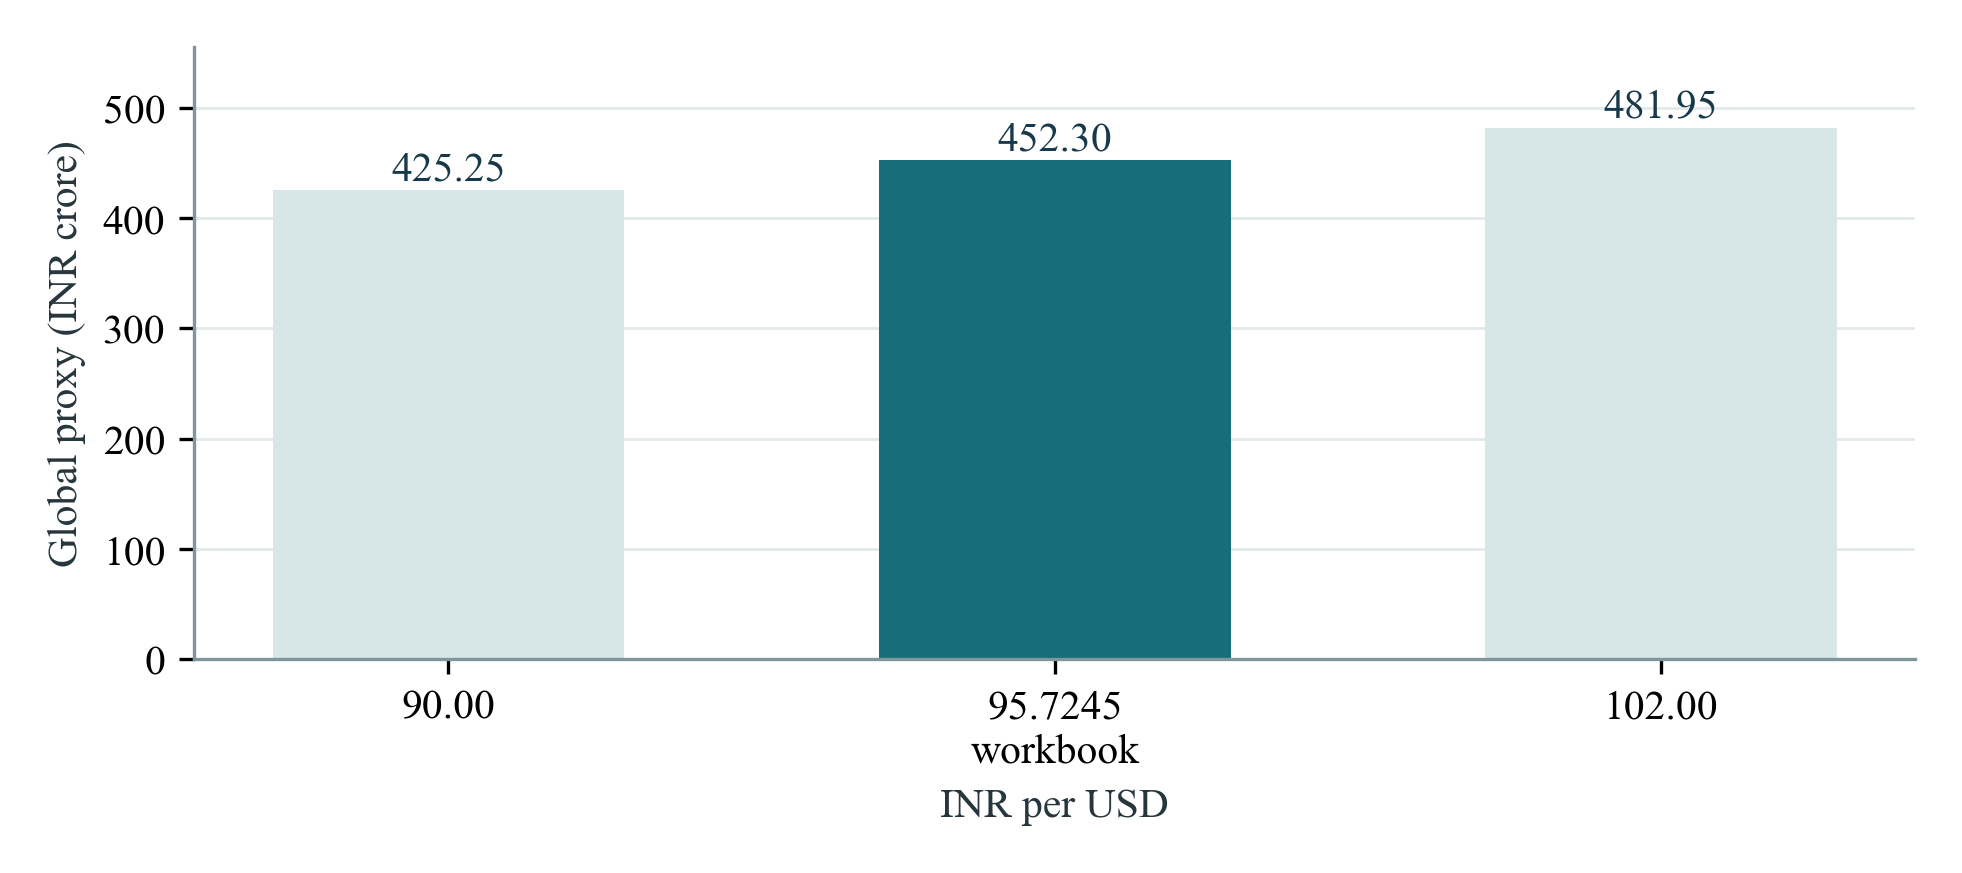
\includegraphics[width=0.90\textwidth]{figures/tam-fx.png}
\caption{Global TAM proxy sensitivity to the translation rate. USD 47.25 million is the published 2025 category estimate; INR rates outside 95.7245 are model scenarios.}
\label{fig:tamfx}
\end{figure}

At INR 90, 95.7245 and 102 per USD, Eq.\ \eqref{eq:tam} gives INR 425.25, 452.30 and 481.95 crore. This interval is a currency translation sensitivity, not a confidence interval on the market report. Differences in market definition, data collection and product boundary may exceed the FX effect.

\section{Indian SAM: Bottom-Up Demand}
India's Deep Ocean Mission has an approved INR 4,077 crore outlay, including underwater technology and robotics \cite{dom}. ADITI was launched with INR 750 crore for 2023--24 through 2025--26 and grants up to INR 25 crore for eligible innovation \cite{aditi}. Sagarmala describes 839 projects worth about INR 5.8 lakh crore through 2035 across ports, connectivity and coastal activity \cite{sagarmala}. These are demand contexts. None is a committed SeaNergy procurement, and none is directly multiplied by a market-share percentage.

\begin{table}[htbp]\centering
\begin{tabularx}{\textwidth}{@{}Yrrr@{}}
\toprule
Potential Indian customer group & Units & ASP, INR lakh & Value, INR crore\\ \midrule
MoES / NIOT research payloads & 24 & 18 & 4.32\\
Navy, Coast Guard and defence innovation & 20 & 25 & 5.00\\
Ports and coastal inspection & 45 & 18 & 8.10\\
Inland waterways, dams and reservoirs & 50 & 15 & 7.50\\
Universities, survey labs and developers & 35 & 20 & 7.00\\ \midrule
\textbf{Five-year serviceable total} & \textbf{174} & -- & \textbf{31.92}\\ \bottomrule
\end{tabularx}
\caption{India SAM. Counts and ASPs are project planning estimates tied to named user classes, not published purchase commitments.}
\label{tab:sam}
\end{table}

\begin{figure}[htbp]\centering
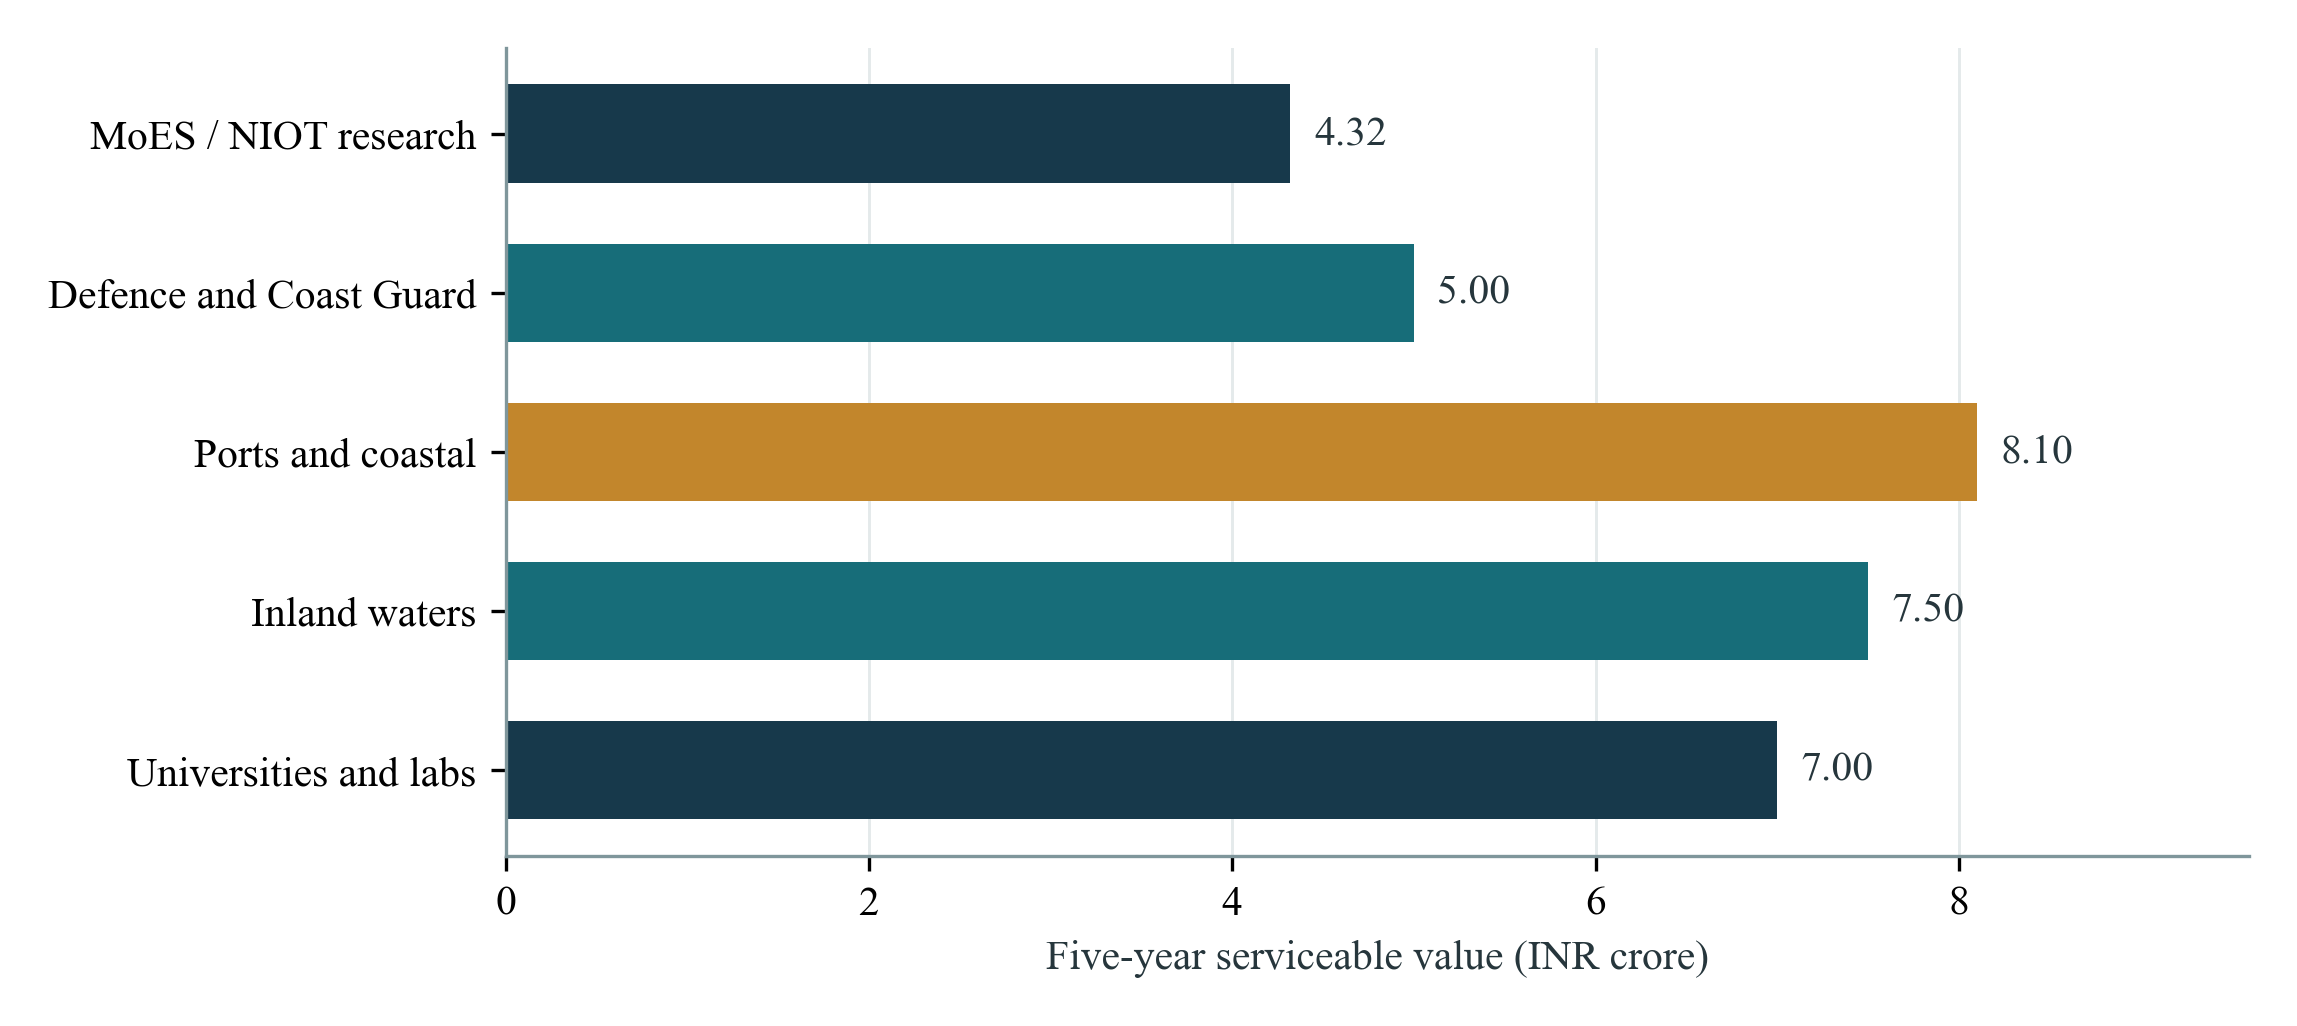
\includegraphics[width=0.91\textwidth]{figures/sam-segments.png}
\caption{Five-year India SAM by customer group, from Table \ref{tab:sam}. Values are INR crore.}
\label{fig:sam}
\end{figure}

The five-year SAM is INR 31.92 crore. The unit count is the main uncertainty. Holding ASPs constant, 70\%, 100\%, and 130\% of the estimated unit opportunities produce INR 22.34, 31.92, and 41.50 crore. These are explicit demand scenarios, not a statistical range. The lower case is useful because public programme activity does not automatically become a budget line for adaptive transmitters. Procurement specifications, demonstration access, qualification and the presence of platform integrators determine whether each opportunity is truly serviceable.

\section{SOM: Qualification-Led Capture}
The workbook stages 35 integrated engagements over five relative years, with ASP rising from INR 15 to 20 lakh as scope and qualification deepen. The first year's INR 15 lakh is an \emph{integrated evaluation programme}, not one INR 1.95 lakh evaluation kit. This interpretation resolves the two-price ambiguity in the source workbook.

\begin{table}[htbp]\centering
\begin{tabularx}{\textwidth}{@{}YrrrY@{}}
\toprule
Year & Units & ASP, INR lakh & Revenue, INR crore & Commercial gate\\ \midrule
Y1 & 1 & 15 & 0.15 & Integrated evaluation\\
Y2 & 3 & 16 & 0.48 & Paid pilots\\
Y3 & 6 & 18 & 1.08 & Qualified pilots\\
Y4 & 10 & 19 & 1.90 & Early scale\\
Y5 & 15 & 20 & 3.00 & Platform / OEM\\ \midrule
\textbf{Five-year} & \textbf{35} & -- & \textbf{6.61} & Scenario\\ \bottomrule
\end{tabularx}
\caption{Staged integrated-programme SOM from the project workbook. Revenue is a planning scenario, not booked sales.}
\label{tab:som}
\end{table}

\begin{figure}[htbp]\centering
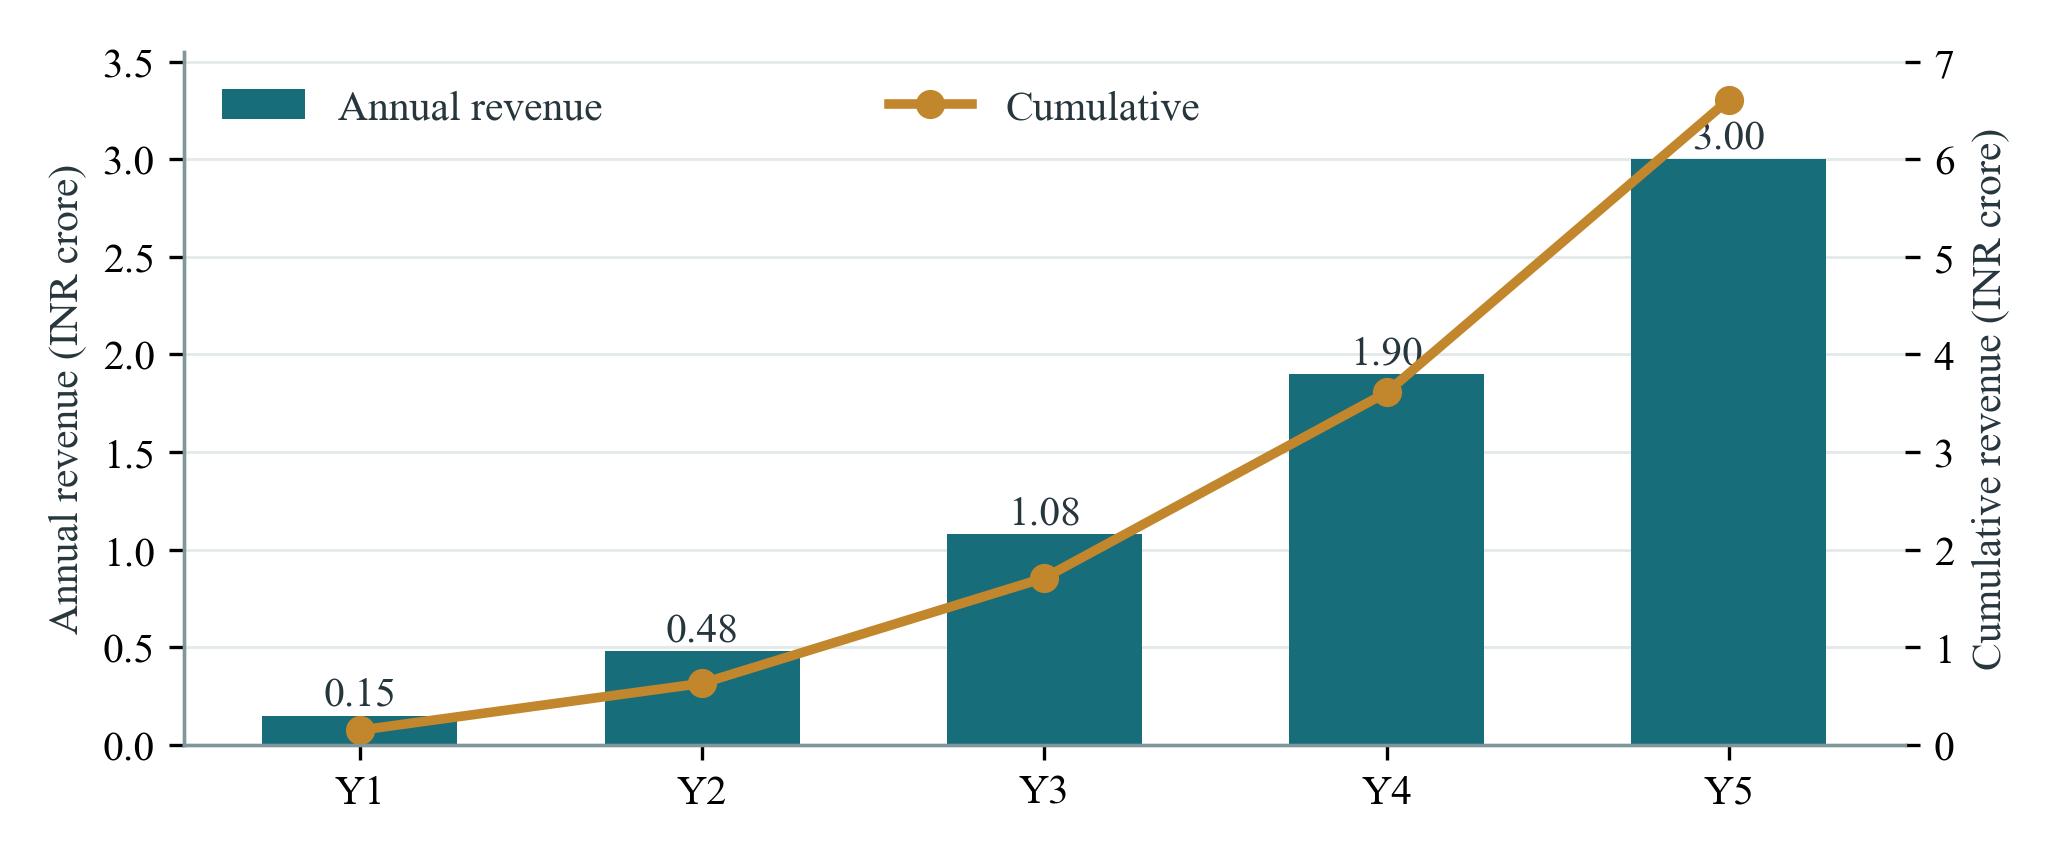
\includegraphics[width=0.92\textwidth]{figures/som-ramp.png}
\caption{Annual and cumulative integrated-programme revenue in the base SOM scenario. Values are INR crore; Y1--Y5 are relative forecast years.}
\label{fig:som}
\end{figure}

The 35 engagements equal 20.1\% of estimated SAM units; INR 6.61 crore equals 20.7\% of SAM value. That is a demanding capture rate for a new hardware platform. A downside case of 18 engagements at INR 16 lakh average yields INR 2.88 crore; an upside case of 45 at INR 20 lakh yields INR 9.00 crore. Neither assumes an awarded tender. A realistic sales funnel requires a named platform partner, qualification samples, calibrated acoustic evidence, field references, and funds for warranty and deployment support.

\section{Engineering Cost Base}
\subsection{Prototype quantity curve}
The hardware quantity model uses the quantity-one BOM, a component discount factor, and quantity-specific PCB, enclosure and assembly allowances \cite{bom}. Its figures are estimates rather than binding Indian supplier quotations.

\begin{table}[htbp]\centering
\begin{tabularx}{\textwidth}{@{}Yrrr@{}}
\toprule
Batch quantity & Unit cost, INR & Batch cost, INR & Reduction vs one\\ \midrule
1 & 27,648 & 27,648 & --\\
10 & 21,751 & 2,17,514 & 21.3\%\\
100 & 17,501 & 17,50,064 & 36.7\%\\ \bottomrule
\end{tabularx}
\caption{Prototype hardware quantity model. Rounded unit values cause small differences from extended batch totals.}
\label{tab:qty}
\end{table}

The demonstration allowance is INR 36,000 for one marine-ready showcase unit, leaving INR 8,352 above the INR 27,648 hardware estimate for freight, quotation movement, machining or print iteration, seals, calibration consumables and contingency \cite{bom}. Laboratory equipment and tank infrastructure are excluded. The quantity-100 cost does not automatically become the evaluation-unit electronics COGS because the scopes and assembly boundaries differ.

\subsection{Evaluation-unit COGS}
\begin{table}[htbp]\centering
\begin{tabularx}{\textwidth}{@{}Yrr@{}}
\toprule
Cost element & INR per unit & Share of COGS\\ \midrule
Electronics and PCB & 26,148 & 22.2\%\\
Enclosure and sealed integration & 18,500 & 15.7\%\\
Transducers & 36,000 & 30.6\%\\
Battery and power & 8,500 & 7.2\%\\
Assembly and calibration & 17,000 & 14.4\%\\
QA and warranty reserve & 8,000 & 6.8\%\\
Packaging and field kit & 3,500 & 3.0\%\\ \midrule
\textbf{Estimated total COGS} & \textbf{1,17,648} & \textbf{100.0\%}\\ \bottomrule
\end{tabularx}
\caption{Evaluation-unit planning COGS, ex-GST. Shares are rounded independently.}
\label{tab:cogs}
\end{table}

\begin{figure}[htbp]\centering
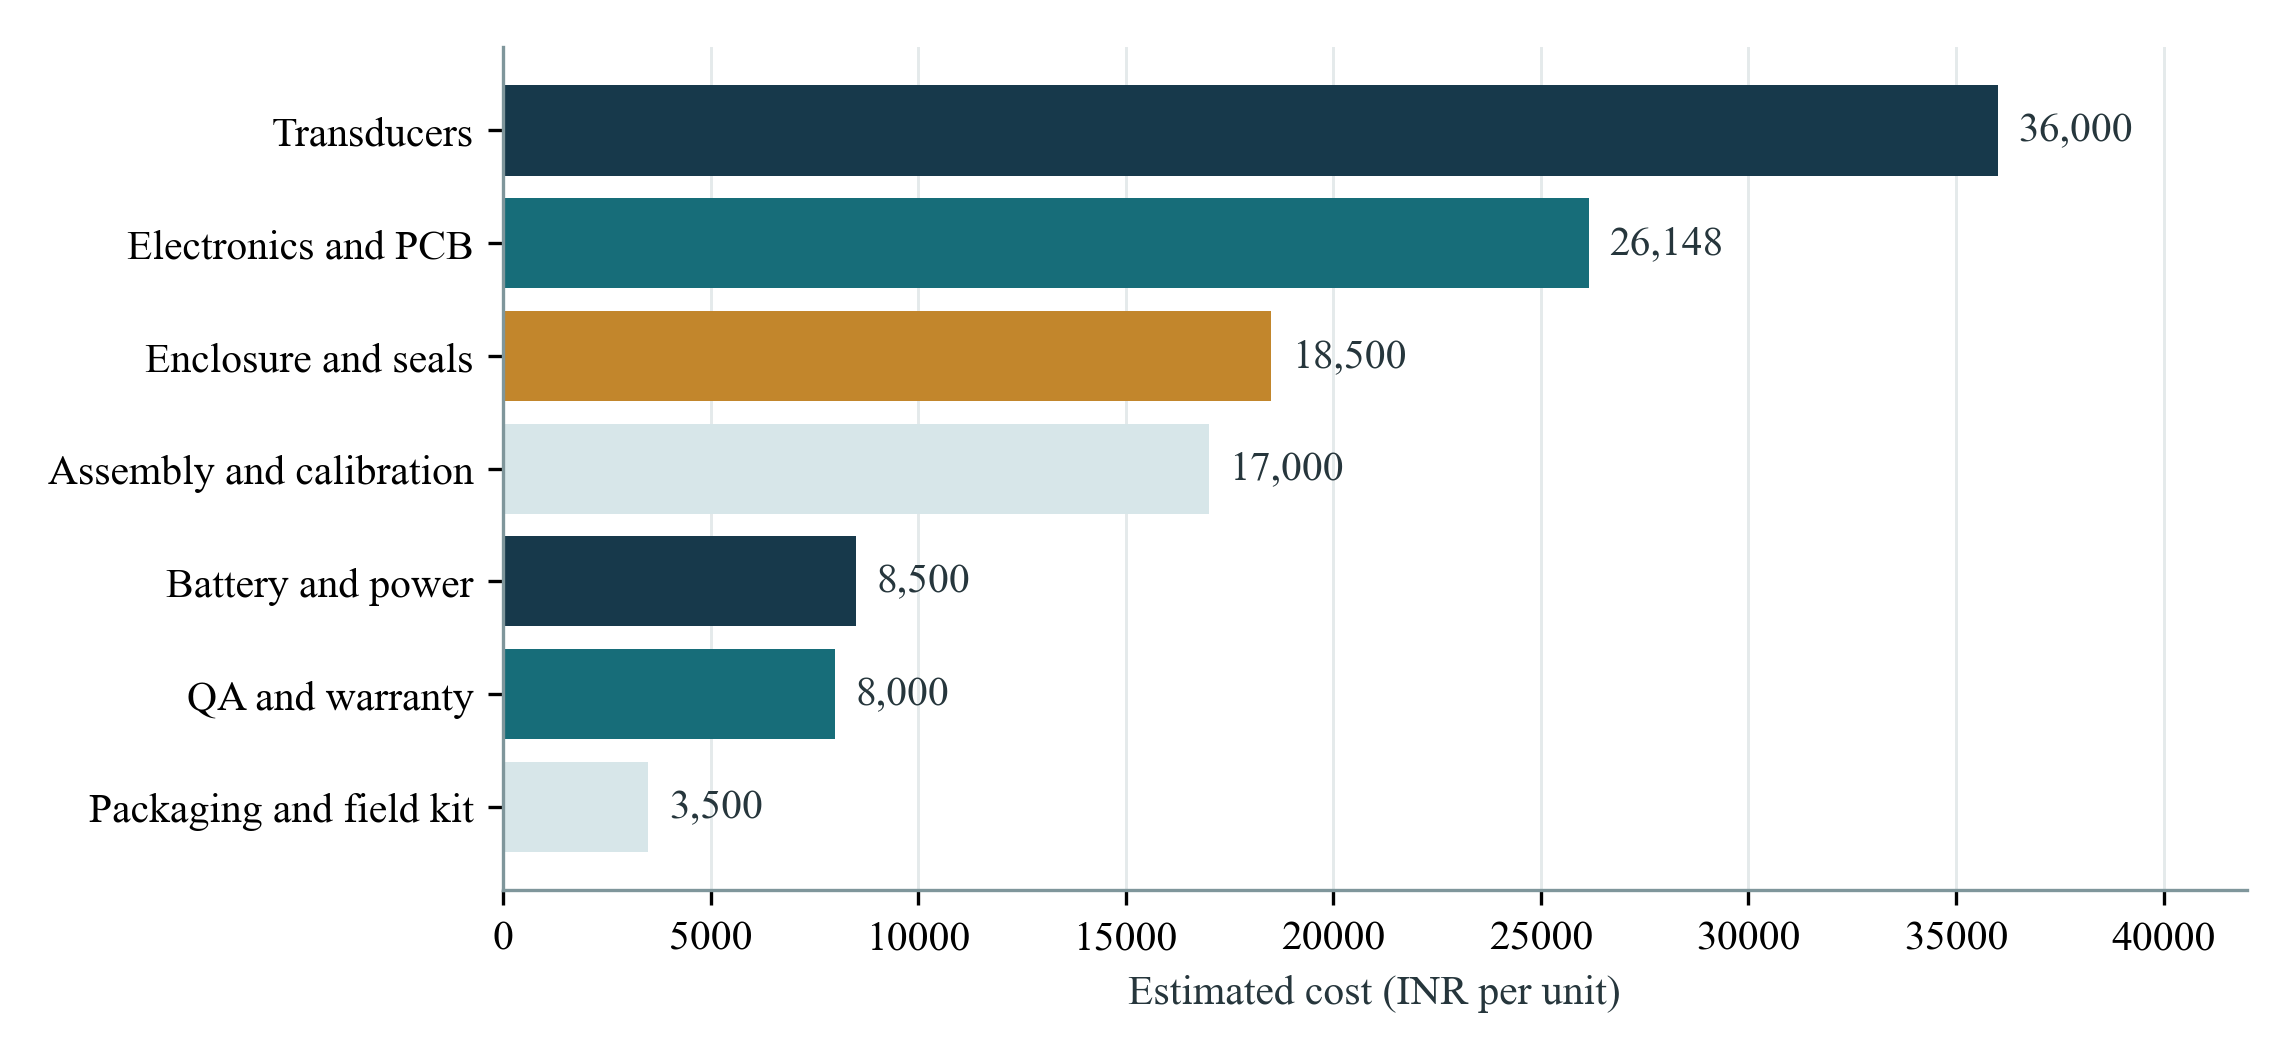
\includegraphics[width=0.88\textwidth]{figures/cogs.png}
\caption{Evaluation-unit COGS composition in INR. Transducers and electronics together account for just over half of the modelled cost.}
\label{fig:cogs}
\end{figure}

The transducer allowance is the largest single line. Airmar's P66 is a real 50/200\,kHz, 600\,W reference option for a later marine integration path \cite{airmar}; final selection needs impedance, mounting and connector verification. A calibrated hydrophone path is also a programme expense, not an ordinary per-unit component. The roadmap reserves INR 7.5 lakh within the field-stage total for the reference hydrophone, conditioning and calibration paperwork \cite{roadmap}. Keeping these categories separate makes the apparent kit margin less misleading.

\section{Price, Gross Margin and Cost Sensitivity}
At target evaluation-unit price $p={\rm INR}\ 1,95,000$ and COGS $c={\rm INR}\ 1,17,648$, gross profit $p-c$ is INR 77,352 and gross margin $(p-c)/p$ is 39.67\%. This includes repeatable assembly and calibration in COGS. It does not include product development, field qualification, sales travel, tender expense, inventory financing, administrative overhead or income tax. It is not a net margin and cannot be applied to the higher ASP integrated programme without its own COGS.

\begin{table}[htbp]\centering
\begin{tabularx}{\textwidth}{@{}Yrrr@{}}
\toprule
Evaluation-unit case & Price, INR & COGS, INR & Gross margin\\ \midrule
Base & 1,95,000 & 1,17,648 & 39.7\%\\
COGS +10\% & 1,95,000 & 1,29,413 & 33.6\%\\
Price -10\% & 1,75,500 & 1,17,648 & 33.0\%\\
Both adverse shifts & 1,75,500 & 1,29,413 & 26.3\%\\ \bottomrule
\end{tabularx}
\caption{Deterministic unit-margin sensitivity. COGS is rounded to the nearest INR for display; calculations use unrounded figures.}
\label{tab:sens}
\end{table}

\begin{figure}[htbp]\centering
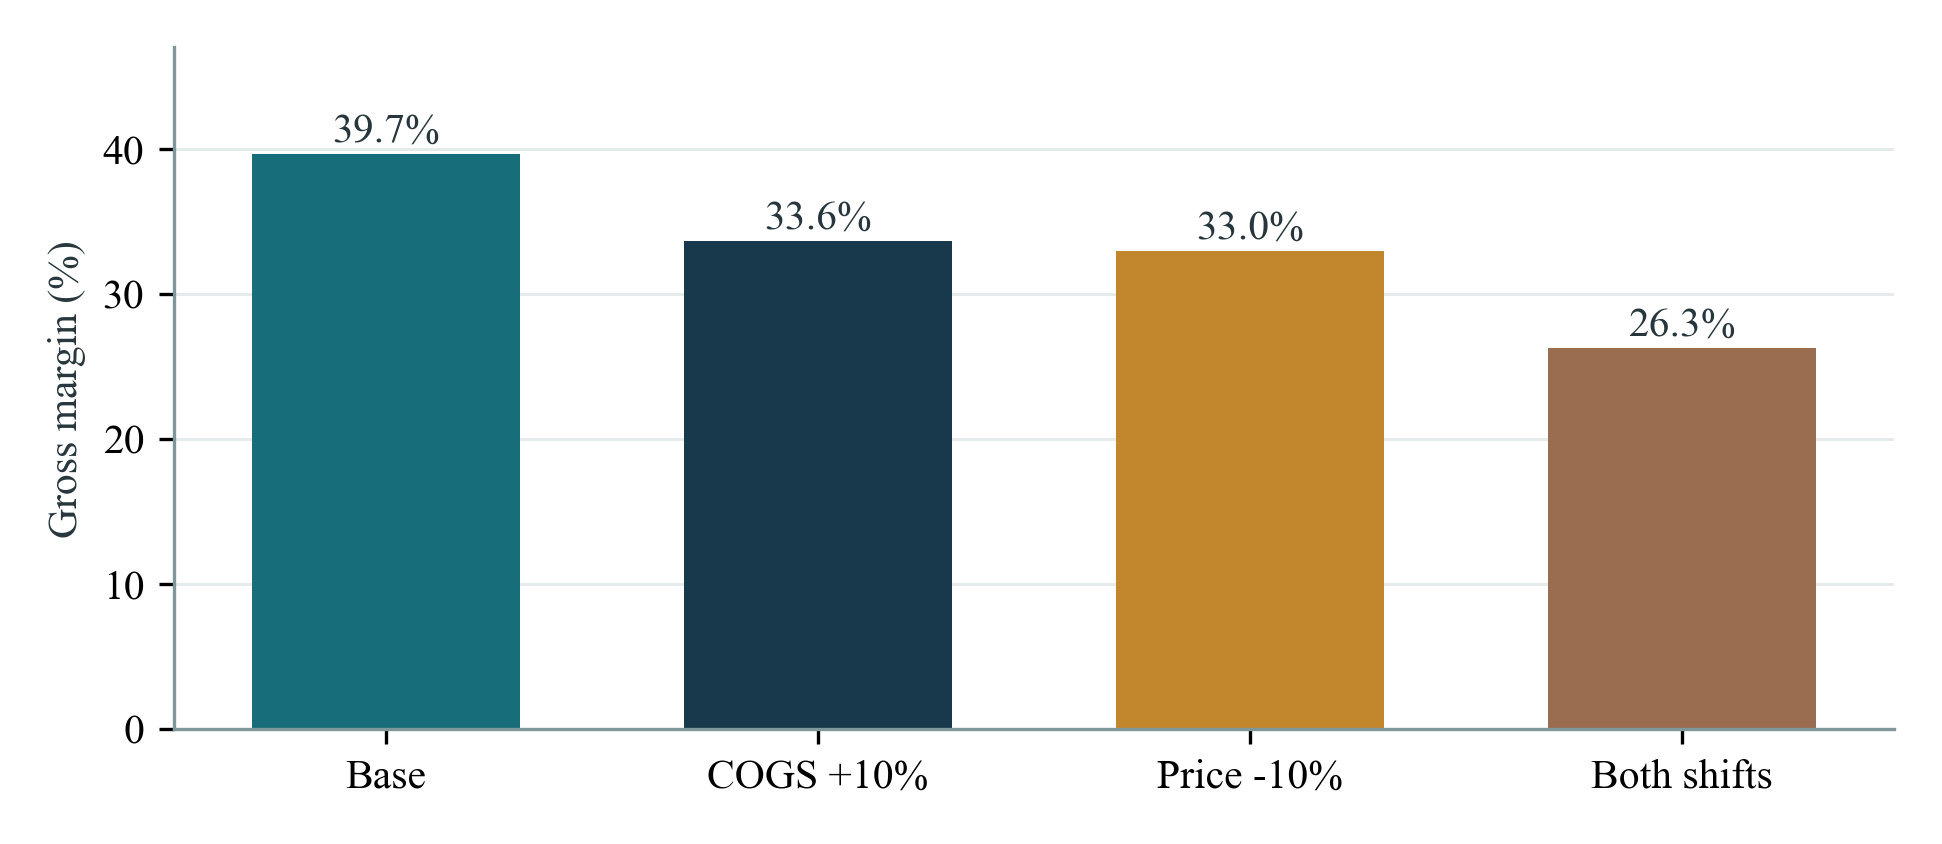
\includegraphics[width=0.89\textwidth]{figures/margin-sensitivity.png}
\caption{Gross-margin sensitivity for the evaluation-unit offer. Price pressure and COGS inflation compound.}
\label{fig:margin}
\end{figure}

A 10-unit evaluation-unit batch ties up roughly INR 11.76 lakh in modelled COGS before receipts, excluding spares and customer-payment delays. Written landed quotations, component lead times, and a procurement log should control the next cost revision. A transducer cost change of INR 2,000 moves COGS and gross profit by the same amount per unit. A second quantity-one enclosure print adds roughly INR 1,200 in the hardware model \cite{bom}.

\section{Development Reserve and Break-Even Check}
The roadmap lists a field-payload scaling reserve of INR 14.35 lakh, including revision-B PCB and assembly, 24\,V/100\,W bridge and protection, production transducer allowance, sealed interfaces, low-noise receive chain, calibrated hydrophone package, pressure housing, and integration contingency \cite{roadmap}. The market workbook separately carries an INR 1,27,190 phase-one IP allowance \cite{workbook}. Their sum is INR 15,62,190. These are programme planning allowances, not per-unit COGS or expenses already incurred.

As a simple stress check, if every sale were the INR 1.95 lakh evaluation unit and each contributed INR 77,352 gross profit, covering the combined allowances would require $\lceil15,62,190/77,352\rceil=21$ units before all other overhead. At 35 evaluation units, gross profit would be INR 27,07,320, leaving INR 11,45,130 after those allowances but before overhead. This is \emph{not} the SOM profit forecast: the actual SOM assumes integrated packages with a different, unpriced cost structure. The check only asks whether the scale of the kit economics can plausibly carry the proposed engineering reserve.

The INR 14.35 lakh reserve is sensitive to calibrated instrumentation and pressure housing. If a laboratory or vehicle integrator supplies that infrastructure, the direct cash requirement falls; if a mission demands additional certification, redesign or specialized testing, it rises. A field quote should separate one-time engineering, recurring hardware, tooling, calibration, warranty and support rather than putting everything into a single payload price.

\section{Competitive Procurement Context}
The public Ping360 list price is USD 2,750, about INR 2.63 lakh at the model FX, before freight, customs, GST and local integration \cite{ping}. The Sonoptix ECHO is listed from USD 8,950, about INR 8.57 lakh on the same basis \cite{echo}. They are complete scanning and multibeam products respectively; SeaNergy's evaluation unit is not feature-equivalent. Their value in this paper is a procurement reference for buyers considering imported acoustic equipment. Comparison should cover acoustic function, range, beam coverage, depth rating, interface, installation and support, not price alone.

SeaNergy's proposed differentiator is a transparent adaptive transmit controller integrated locally. A buyer may still need a separate receive chain, transducer, pressure enclosure, navigation integration and survey software. The local proposition becomes strongest when an OEM or research AUV team already has those elements and wants programmable waveform control. It is weaker where the buyer needs a ready-made imaging system with an established field track record.

\section{Risk, Evidence and Next Price Revision}
The main market risk is that a published global category and national technology programmes are broader than the actual market for one adaptive transmitter. The main capture risk is a long qualification cycle. The main cost risk is treating prototype supplier listings as landed production prices. The main technical-economic risk is that energy, SFDR, acoustic source level, enclosure rating and receive protection require additional engineering before a production offer. The research paper provides bounded team-reported spectral and energy figures; pricing should fund the work needed to close those gaps.

Before quoting an integrated package, the team should obtain at least two landed transducer quotations, an assembly and sealed-housing quotation, a calibrated measurement plan, a warranty-return assumption, and a vehicle integrator's acceptance criteria. The revised workbook should preserve versioned assumptions, quote dates, currency rate, quantity breaks, and tax treatment. Market counts should be linked to named organizations or specific tenders as discovery proceeds. A government programme outlay may indicate strategic relevance but is never counted as a sale.

\section{Conclusion}
The current model supports a credible first commercial discussion if its boundaries remain visible. A narrow published global category translates to INR 452.30 crore at the stated rate. Bottom-up Indian opportunities total an estimated INR 31.92 crore over five years; the staged INR 6.61 crore obtainable scenario is ambitious and qualification-dependent. An INR 1.95 lakh evaluation unit has estimated INR 1,17,648 COGS and 39.7\% gross margin before programme overhead. The integrated payload revenue scenario has a different cost structure and needs its own quotation. The most useful next evidence is not a larger top-down market number; it is a calibrated field demonstration, named customer discovery, and repeatable landed cost.

\appendix
\section{Audit Trail and Calculation Detail}
\begin{table}[htbp]\centering
\begin{tabularx}{\textwidth}{@{}p{0.25\textwidth}Y@{}}
\toprule
Reported number & Formula and source\\ \midrule
INR 452.30 crore TAM & USD 47.25 million times 95.7245 INR/USD divided by 10 \cite{diresearch,fx}\\
INR 31.92 crore SAM & Sum of five row products in Table \ref{tab:sam} \cite{workbook}\\
INR 6.61 crore SOM & Sum of Y1--Y5 row products in Table \ref{tab:som} \cite{workbook}\\
39.7\% kit margin & $(1,95,000-1,17,648)/1,95,000$ \cite{workbook}\\
21-unit allowance check & Ceiling of 15,62,190 divided by 77,352\\
INR 2.63 and 8.57 lakh benchmarks & USD 2,750 and 8,950 times 95.7245, before import charges \cite{ping,echo,fx}\\ \bottomrule
\end{tabularx}
\caption{Arithmetic and cited inputs for figures most likely to be reused in a presentation.}
\end{table}

\section{Interpretation Rules}
TAM is a global adjacent-category proxy, not SeaNergy's obtainable revenue. SAM is an estimated five-year Indian serviceable opportunity count times integrated ASPs. SOM is a staged capture scenario within SAM, not contracted revenue. Prototype BOM is neither evaluation-unit COGS nor the full integrated-package COGS. Gross margin excludes development, qualification, sales and overhead. Public supplier prices are list prices, not landed Indian quotations. The FX input is fixed for comparability and must be updated with a date when a new offer is issued.

\begin{thebibliography}{99}\small
\bibitem{diresearch} DIResearch, \emph{Global Side Scan Sonars Market Research Report 2025--2032}, published 10 July 2025. \href{https://www.marketresearch.com/Deep-Insights-Research-Co-DIR-v4285/Global-Side-Scan-Sonars-Research-41780036/}{Report summary}.
\bibitem{gir} Global Info Research, \emph{Global Side Scan Echo Sounder Market 2026--2032}, published 31 July 2026. \href{https://www.marketresearch.com/GlobalInfoResearch-v4117/Global-Side-Scan-Echo-Sounder-45818082/}{Report summary}.
\bibitem{fx} Metropolitan Stock Exchange of India, \emph{RBI Reference Rate Archives}, INR 95.7245/USD used by project workbook for 11 September 2026. \href{https://www.msei.in/markets/currency/historical-data/rbireferenceratearchives}{Archive}.
\bibitem{dom} Press Information Bureau, Government of India, \emph{Cabinet approves Deep Ocean Mission}, 2021. \href{https://www.pib.gov.in/PressReleasePage.aspx?PRID=1727526&lang=2&reg=48}{Official release}.
\bibitem{aditi} Press Information Bureau, Ministry of Defence, \emph{DefConnect 2024: ADITI scheme}, 4 March 2024. \href{https://www.pib.gov.in/Pressreleaseshare.aspx?PRID=2011171&lang=2&reg=48}{Official release}.
\bibitem{sagarmala} Ministry of Ports, Shipping and Waterways, \emph{Projects Under Sagarmala}, project dashboard. \href{https://sagarmala.gov.in/projects/projects-under-sagarmala}{Official page}.
\bibitem{ping} Blue Robotics, \emph{Ping360 Scanning Imaging Sonar}, public list price USD 2,750, accessed 26 September 2026. \href{https://bluerobotics.com/store/sonars/imaging-sonars/ping360-sonar-r1-rp/}{Product page}.
\bibitem{echo} Blue Robotics, \emph{Sonoptix ECHO Multibeam Imaging Sonar}, public starting price USD 8,950, accessed 26 September 2026. \href{https://bluerobotics.com/store/sonars/imaging-sonars/sonoptix-echo/}{Product page}.
\bibitem{airmar} Airmar Technology, \emph{P66 transducer catalog}, 50/200 kHz and 600 W specifications. \href{https://www.airmartechnology.com/uploads/catalogPages/cat_55.pdf}{Catalog}.
\bibitem{bom} Hyper Grey, \emph{SeaNergy quantity cost model and purchase BOM}, repository \texttt{01-hardware/bom/}, 2026.
\bibitem{workbook} Hyper Grey, \emph{SeaNergy cost-model.xlsx}, repository \texttt{09-business/market/}, 2026.
\bibitem{roadmap} Hyper Grey, \emph{SeaNergy scaling analysis}, repository \texttt{09-business/roadmap/scaling-analysis.md}, 2026.
\end{thebibliography}
\end{document}
